\chapter{Introducción}
\section{Introducción}
Uno de los problemas que se plantea en la actualidad en el proceso de enseñanza-aprendizaje es la cantidad de alumnos que están en una misma aula a cargo de un solo docente. Este aspecto es uno de los más debatidos en la educación. \cite{PANORAMA2018}

Según \citeA{LILIA2013}, la superpoblación estudiantil es el exceso del número de estudiantes que se encuentran en un espacio determinado cuya capacidad no es adecuada para acogerlos ni cuenta con las condiciones adecuadas para el buen desenvolvimiento de los mismos.

En el caso particular de España, el tamaño de clase medio en Educación Secundaria en las instituciones públicas es superior al promedio de la OCDE y de la UE22. \cite{PANORAMA2018}

Esto no implica que en todos los casos en el que la ratio sea superior exista una sobrepoblación, sin embargo, la calidad educativa se ve mermada por esta situación.

\begin{figure*}[htb]
	\centering
	\caption{Número medio de alumnos por clase en instituciones públicas (2016). Recuperado del \protect\citeA{PANORAMA2018}}
	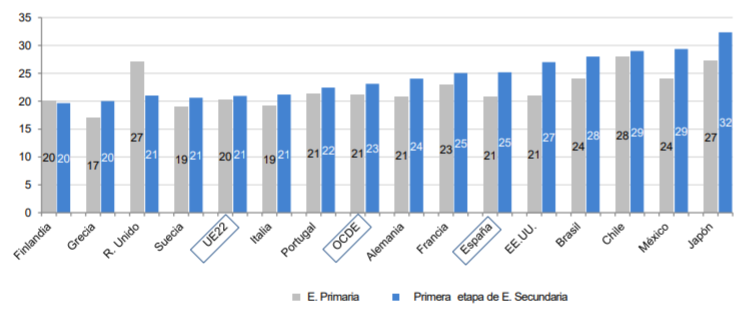
\includegraphics[width=0.8\textwidth]{recursos/NumeroAlumnosClase}
	\label{fig:NumeroAlumnosClase}
\end{figure*}
\FloatBarrier

En la figura \ref{fig:NumeroAlumnosClase} se puede observar como la media del número de alumnos por clase de la Unión Europea está en 21 alumnos para la etapa de Secundaria, mientras que en España la media asciende a 25 alumnos.

Si bien es cierto, que es bueno que se deba atender a la diversidad y a la inclusión (sobre el número de alumnos) en el aula, esto debe hacerse de forma responsable y conociendo las limitaciones que tiene el docente, que por más voluntad o capacitación que posea, tiene que atender a las necesidades personalizadas de cada alumno. \cite{HILDA2014}

\citeA{lera2007calidad} en su articulo se plantea la reducción del numero de alumnos o el aumento de asistentes en el aula con el objetivo de mejorar la calidad educativa. 

La ratio, que es la relación entre el número de alumnos y profesores, es un factor importante a la hora de realizar la planificación de los recursos. En el año 2012, dicho ratio, en España aumentó un 20\%, lo que implica un ahorro en torno a 464 millones de euros. Aprobado por el Real Decreto-ley 14/2012 en el artículo 2.

Debido a que los recursos de una administración no son infinitos, es necesario tener en cuenta los recursos disponibles para la educación; concretamente, durante 2015 España presenta un gasto total por alumno inferior al promedio de los países de la OCDE y la UE22. Véase la figura \ref{fig:procPerformance}. Esto implica que se dispone de menos recursos en la educación y por lo tanto se tiende a agrupar a los alumnos en grupos de mayor tamaño.

\begin{figure*}[htb]
	\centering
	\caption{Gasto total anual (2015). Recuperado del \protect\citeA{PANORAMA2018}}
	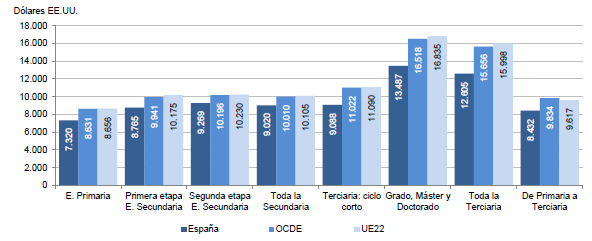
\includegraphics[width=0.8\textwidth]{recursos/GastoEducacion}
	\label{fig:procPerformance}
\end{figure*}
\FloatBarrier

Por las razones anteriormente comentadas, es importante establecer una buena gestión sobre los recursos disponibles, realizando una óptima distribución tanto de los docentes como de los recursos asignados a estos.

\begin{comment}
En los últimos años, gracias al gran desarrollo tecnológico que se ha vivido tanto a nivel de computo (mejorando la eficiencia y el uso de los recursos disponibles) como a nivel de transmisión de datos (mejorando las comunicaciones), ha permitido a las organizaciones el almacenamiento de una gran cantidad de información.

Para comprender mejor este gran volumen de información que disponen las organizaciones, es necesario utilizar métodos, técnicas, herramientas además de personas con conocimientos (formando todas esta un vínculo estrecho) que permita y ayude a explotar, investigar, predecir y obtener información relevante para tomar decisiones de forma adecuada.

Para descubrir la información en estos grandes volúmenes de datos, es necesario abordar el concepto de minería de datos.  Según \citeA{martinez2016mineria}, la minería de datos es el ``proceso que permite transformar información en conocimiento útil para el
negocio, a través del descubrimiento y cuantificación de relaciones en una
gran base de datos". La minería de datos aplica técnicas estadísticas y matemáticas para poder obtener esta información implícita en los datos.

Algunas de las aplicaciones de la minería de datos según \cite{riquelme2006mineria} son:  comercio y banca, medicina y farmacia, seguridad y detección de fraude, astronomía, geología, minería, agricultura, pesca, ciencias ambientales y ciencias sociales.


\section{Contexto}
Las organizaciones de ámbito educativo no han quedado ajenas a estas necesidades de una mejor comprensión de los datos. Según \citeA{romero2010educational} la minería de datos educativa (EDM) se encarga del desarrollo de métodos para explotar los datos del entorno educativo y entender mejor a los estudiantes y las herramientas que se utilizan para el aprendizaje de estos.

Por un lado, tanto el software educativo como las bases de datos institucionales, han generado una gran cantidad de datos acerca de alumnos, reflejando el aprendizaje de estos a lo largo del tiempo. Por otro, el uso pedagógico de Internet (eLearning), ha generado también grandes cantidades de datos acerca de la enseñanza-aprendizaje (técnicas, herramientas, etc). "Toda esta información es una mina de oro, en el contexto educativo". \cite{romero2010educational}.

\citeA{MOHAMAD2013320} define EDM como una disciplina emergente, relacionada con el desarrollo de métodos para la explotación de datos que proceden del entorno educativo, para entender mejor a los estudiantes y las herramientas que estos utilizan para aprender. Coincide con el artículo de \citeA{inbook} en el que se indica que la EDM se ha desarrollado más lentamente que en el resto de ámbitos.

Como se puede observar en el artículo de \citeA{sin2015application} y en la figura \ref{fig:artPublicados}, el número de artículos publicados en la conferencia internacional sobre la minería de datos ha crecido desde 2011 casi exponencialmente.

Este aumento de artículos publicados muestra como existe un aumento en el uso de la minería de datos en la educación.

\begin{figure*}[htb]
	\centering
	\caption{Artículos aceptados y publicados desde 2011. Recuperado de \protect\citeA{sin2015application}}
	\includegraphics[width=0.6\textwidth]{recursos/artPublicados}
	\label{fig:artPublicados}
\end{figure*}
\FloatBarrier

A su vez, \citeA{sin2015application}, ha categorizado los artículos publicados según su contenido en categorías que definen las distintas aplicaciones de la minería de datos en la educación. Algunas de estas categorías son: detección de comportamiento, estimación de habilidades, predicción de mejora académica, etc. Por tanto, como se puede observar, dentro de la minería de datos en el entorno educativo, existen distintos campos estudiados y distintos ámbitos de aplicación.
\end{comment}

\section{Objetivos} 
\label{objetivos}
En este trabajo fin de máster (TFM) se expone una solución a la necesidad que tiene la Consejería de Educación e Investigación de la Comunidad de Madrid (CEI) para dar respuesta a las necesidades de la demanda concreta de plazas escolares de un nuevo período escolar. Para ello, se plantea el uso de herramientas y métodos flexibles que automaticen las tareas de planificación y proponga, además, nuevas variables o factores que puedan influir en la toma de decisiones. 

El interés que justifica este TFM es avanzar en el conocimiento sobre los factores del entorno educativo que implican el aumento de la superpoblación de un aula. De esta manera, se consigue que las Unidades (que tienen la competencia de gestionar la demanda de plazas escolares de un nuevo periodo escolar) tengan mayor facilidad a la hora de implantar un Sistema que sea capaz de predecir el número de grupos, a partir de los factores disponibles en cursos previos.

Las consideraciones que se han realizado en los párrafos anteriores justifican que el objetivo general de este TFM es: proponer un modelo para contribuir a la óptima planificación de los grupos escolares para los nuevos cursos, evitando así el gasto innecesario de recursos y controlando la sobrepoblación en el aula.

Dicho objetivo global se pretende alcanzar mediante los siguientes sub objetivos:
\begin{itemize}
	\item Seleccionar variables de interés, relativas a la resolución de la necesidad anteriormente expuesta por Unidad de Planificación, que aporten valor en el desarrollo de este TFM. %MODIFICAR
	\item Estudiar la relación entre dichas variables con el propósito de comprender el contexto de la sobrepoblación en el aula y la planificación de grupos.
	\item Probar distintos modelos predictivos y seleccionar aquellos que aporten mayor precisión en la predicción de los grupos. 
	\item Obtener y utilizar el modelo de mayor precisión para realizar predicciones con los datos existentes en el entorno educativo de la Comunidad de Madrid en los últimos 10 años y que este modelo ayude a las Unidades de la CEI a planificar grupos en los nuevos cursos. 
\end{itemize}

\section{Metodología}
El proceso o metodologia llevado a cabo en este TFM sigue las siguientes fases:
\begin{enumerate}
	\item En primer lugar, se detecta la necesidad ya expuesta por la Unidad de la Consejería de Educación e Investigación de la Comunidad de Madrid\footnote{El autor de este TFM ha colaborado con la Consejería de Educación e Investigación de la Comunidad de Madrid en el desarrollo de un proyecto (ALAS) sobre explotación de datos educativos coordinado por la Universidad Politécnica de Madrid, a lo largo del año 2018.}.
	\item Una vez detectada la necesidad, se realizan reuniones con dicha Unidad para obtener la máxima información posible acerca de las necesidades concretas y la forma de satisfacerlas. \footnote{Antes de comenzar la investigación, se debe tener un claro conocimiento sobre las necesidades existentes y se debe establecer un plan de acción.}
	\item Teniendo en cuenta el conocimiento sobre cuáles son las necesidades, se realiza una propuesta\footnote{Esta propuesta es un documento técnico donde se indica qué metodologías se van a emplear para llevar a cabo la investigación, qué modelos predictivos se van a considerar y fundamentalmente cuales son las variables que se van a usar en la predicción (teniendo en cuenta las necesidad de la Unidad de Planificación).} que incluya modelos, variables, y herramientas a la Unidad de Planificación para poder satisfacerlas.% una propuesta que incluya ...
	\item Después de varias reuniones con la Unidad de Planificación, esta Unidad valida la propuesta.
	\item Una vez validada la propuesta, se estudian distintos modelos de predicción a partir de los datos seleccionados en dicha propuesta. Se debe analizar cuál de estos modelos es el que mayor precisión obtiene.
	\item Se decide, en una reunión con la Unidad de Planificación de Centros, cual es el modelo óptimo (teniendo en cuenta la precisión y el tiempo de entrenamiento de los modelos). 
	\item A partir del modelo acordado, se realizan predicciones con los datos de la Unidad.
\end{enumerate}

\section{Organización del TFM}
La estructura que se va a seguir en el TFM es la siguiente:
\begin{itemize}
	\item \textbf{Capítulo 1. Introducción:} En el primer capítulo se definen las necesidades existentes que justifican el desarrollo de este trabajo. También se definen los objetivos que se persiguen con el desarrollo de este. Por último, se presenta la estructura que tiene el presente documento.
	\item \textbf{Capítulo 2. Justificación teórica:} En este segundo capítulo se realiza una investigación sobre el estado de la cuestión, estudiando los métodos, modelos y usos de la minería de datos en el ámbito educativo. 
	\item \textbf{Capítulo 3. Propuesta de intervención:} En este capítulo se define el problema existente.
	\item \textbf{Capítulo 4. Diseño de la investigación:} Este capítulo establece los pasos que se siguen en la realización de un proyecto de minería de datos. Se detallan también las tareas que se van a desempeñar en cada uno de los pasos.
	\item \textbf{Capítulo 5. Análisis de los resultados:} Una vez realizado el análisis exploratorio y predictivo, se mostrarán los resultados obtenidos en este capítulo.
	\item \textbf{Capítulo 6. Conclusiones:} En este capítulo se detallan las conclusiones obtenidas a partir de los resultados alcanzados y los objetivos establecidos.
\end{itemize}
